\chapter{Introduction}
\label{sec:introduction}

\section{Motivation}
Hybrid VTOLs are particularly interesting vehicle to study, which has an intermediate mode as either a Multirotor, or a Fixed Wing.

\begin{figure}[h]
\centering
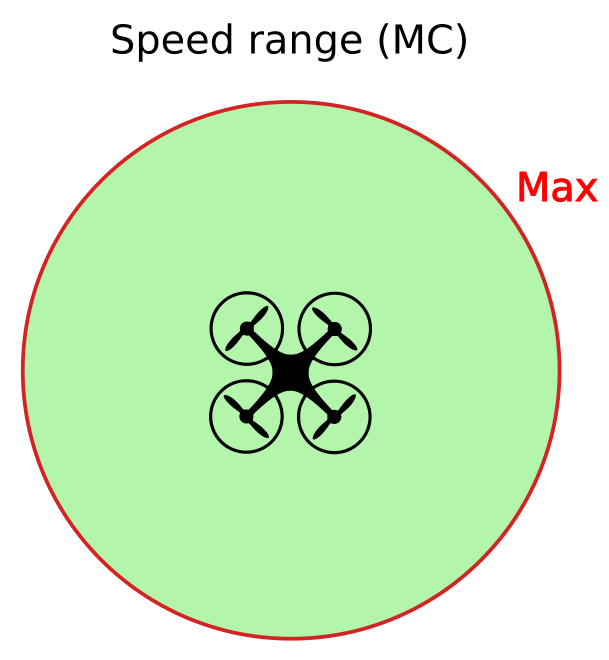
\includegraphics[width=0.3\textwidth]{MC_Velocity_Range}
\caption{Multirotor velocity range}
\end{figure}

\begin{figure}[h]
\centering
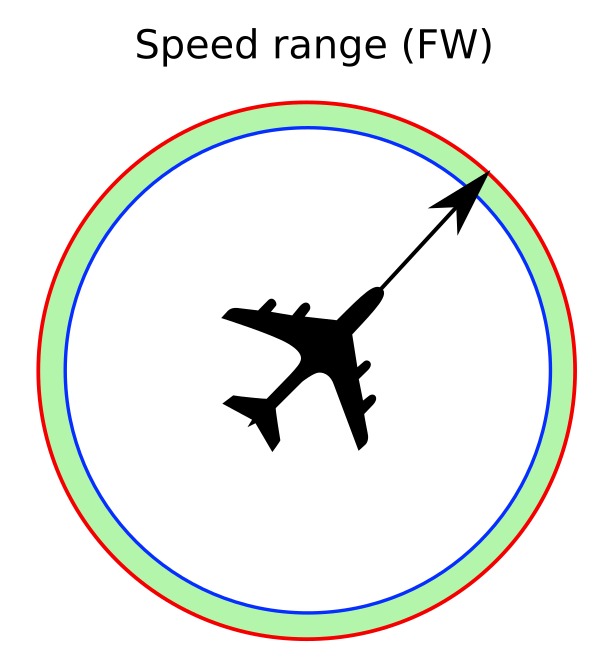
\includegraphics[width=0.3\textwidth]{FW_Velocity_Range}
\caption{Fixed Wing velocity range}
\end{figure}

\section{Goal of this Project}
The goal of this thesis is to construct a unified path following guidance that can be utilized both by Multirotor and Fixed Wing vehicles, thereby also allowing the usage on Hybrid VTOL vehicles.

\section{Contributions}
This thesis, to our best knowledge, describes the first unified path following guidance that specifically accounts for the maneuverability envelope of a Hybrid VTOL.

\section{Overview}
This thesis is structured as following:

\begin{enumerate}
    \item In Problem Definition, we examine the path following problem in detail, and come up with the terminologies as well as the constraints that needs to be respected
    \item In Methods, we present 3 different formulations including the base method (from a past publication) and discuss the differences between them
    \item In Evaluation, we evaluate the formulations against the constraints and desired characteristics defined before
    \item In Conclusion, we determine which formulation is the best, and the use cases based on the evaluation
\end{enumerate}